\documentclass{article}

% if you need to pass options to natbib, use, e.g.:
% \PassOptionsToPackage{numbers, compress}{natbib}
% before loading nips_2016
%
% to avoid loading the natbib package, add option nonatbib:
% \usepackage[nonatbib]{nips_2016}

% \usepackage[final]{nips_2016}

% to compile a camera-ready version, add the [final] option, e.g.:
\usepackage[final]{nips_2016}

\usepackage[utf8]{inputenc} % allow utf-8 input
\usepackage[T1]{fontenc}    % use 8-bit T1 fonts
\usepackage{hyperref}       % hyperlinks
\usepackage{url}            % simple URL typesetting
\usepackage{booktabs}       % professional-quality tables
\usepackage{amsfonts}       % blackboard math symbols
\usepackage{nicefrac}       % compact symbols for 1/2, etc.
\usepackage{microtype}      % microtypography

\usepackage{graphicx}
\graphicspath{ {tu/} }

\usepackage{caption}
\usepackage{subcaption}

\title{On-hands Study of Tree-based Methods}

% The \author macro works with any number of authors. There are two
% commands used to separate the names and addresses of multiple
% authors: \And and \AND.
%
% Using \And between authors leaves it to LaTeX to determine where to
% break the lines. Using \AND forces a line break at that point. So,
% if LaTeX puts 3 of 4 authors names on the first line, and the last
% on the second line, try using \AND instead of \And before the third
% author name.

\author{
  Chenyang~DONG\\
  Department of Mathematics\\
  \texttt{cdongac@connect.ust.hk} \\
  \And
  Tsz Cheung~LO\\
   Department of Computer Science\\
  \texttt{tcloaa@connect.ust.hk} \\
  \And
  Jiacheng~XIA\\
   Department of Computer Science\\
  \texttt{jxiaab@connect.ust.hk} \\
  %% examples of more authors
  %% \And
  %% Coauthor \\
  %% Affiliation \\
  %% Address \\
  %% \texttt{email} \\
  %% \AND
  %% Coauthor \\
  %% Affiliation \\
  %% Address \\
  %% \texttt{email} \\
  %% \And
  %% Coauthor \\
  %% Affiliation \\
  %% Address \\
  %% \texttt{email} \\
  %% \And
  %% Coauthor \\
  %% Affiliation \\
  %% Address \\
  %% \texttt{email} \\
}

\begin{document}
% \nipsfinalcopy is no longer used

\maketitle

\begin{abstract}
Intentionally left blank
\end{abstract}

\section{Introduction}

For the past few lectures we have gone through more methods for doing regression and classification analysis. Among them we decided to go for a study on tree-based methods for the second mini-project. We use tree-based methods both on the America Crime Dataset and the In-class Kaggle competitions, and we find that tree-based methods are straightforward to implement and can give satisfying performance. In this report we present the results for both tests.

The rest of the report is organized as following: Section \ref{crime-Lasso} describes the crime dataset and our previous results in project 1 using Lasso, and make comparisons between Lasso and tree-based methods. Section \ref{combodrug} describes how we used tree-based methods for combinatoric-valued drug data, their results and model comparisons. Section \ref{drug2} presents our results on the in-class Kaggle Competition: Binary OneDrug Data. In the end there is a concluding part summarizing our findings and comments on tree-based methods.

\section{Crime Dataset and Previous Results}
\label{crime-Lasso}
In this section we present the tree based analysis for the crime data. Firstly we describe of the results using regression tree analysis and further optimized by bagging and boosting. In the end the results were compared with Lasso which we used on same dataset for project 1.

\subsection{The American Crime Dataset}
\label{crime_data}
This dataset contains the statistics of crime rate of 7 types in American cities from 1970 to 1992. Besides the name and abbreviation attributes there are 23 features like city population size, number of police, income per capita etc. There are more than 1000 valid data with complete information in this form. Since the features are of different scales, we preprocessed the data by first centering it along the axis to the mean, and component-wise scaling to unit variance.
\subsection{Mini-Project 1 Results}
In the first mini-project, we used various methods to analyze the crime data, and we found that Lasso does best in terms of both prediction and feature selection. Since the seven kinds of crimes are analyzed seperately, we focus on the crime type "Larceny" and we observed that other crime types gave similar results. Lasso gave a test set mean-squared-error (MSE) for around 0.06. We would use this as a benchmark.

\subsection{Regression Tree Analysis}
\label{crime_reg_tree}
We first did a regression tree analysis from the tree analysis. We randomly split 90\% of the data as training set and rest as testing set and got a mean-squared error as 0.1157. As we can see in the graph, regression tree also did well in feature selection, picking out city population, age structure and police forces, which is consistent with our conclusion in project 1.
\begin{figure}[h]
  \centering
  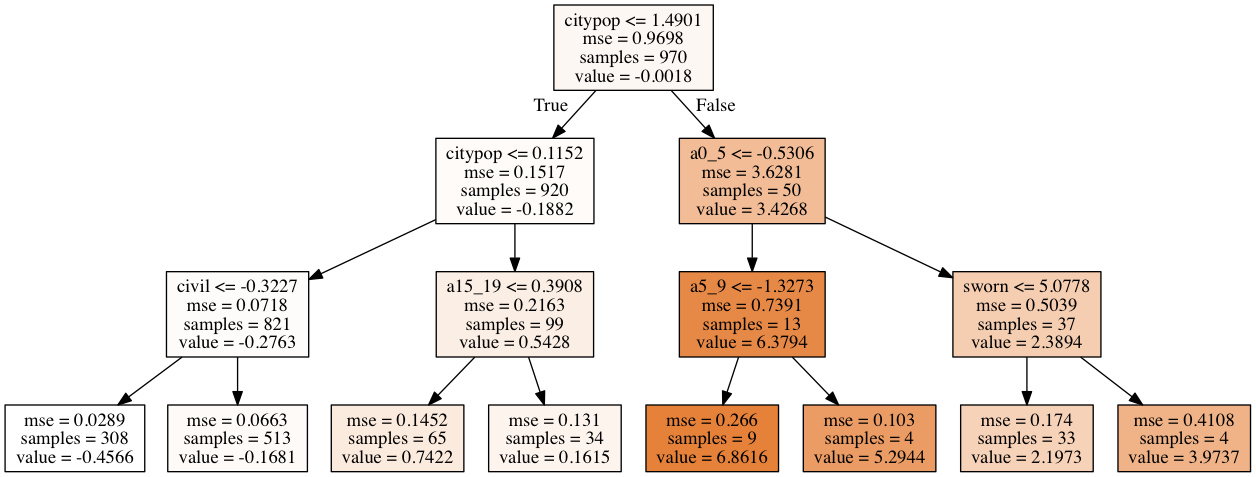
\includegraphics[width=10cm, height=4cm]{crime_treetu}
  \caption{Regression tree on crime data}
\end{figure}

\begin{figure}
\centering
\begin{minipage}{.5\textwidth}
  \centering
  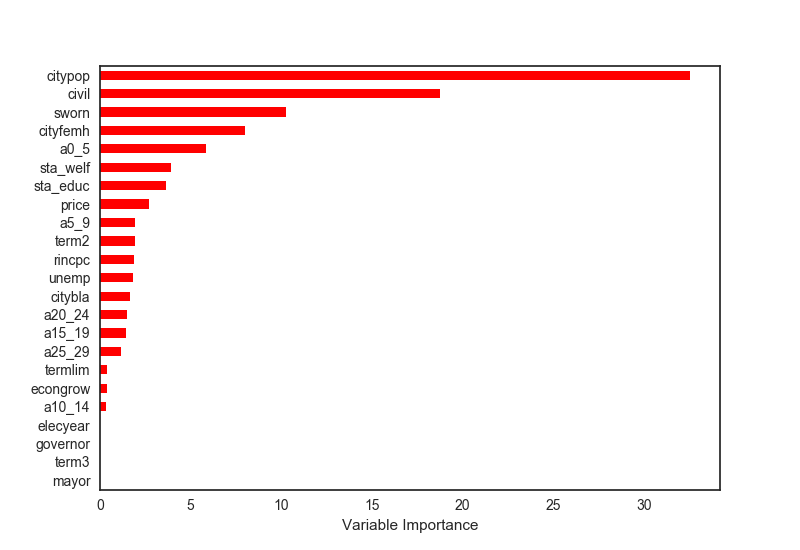
\includegraphics[width=.8\linewidth,height=4cm]{crime_boosttu}
  \captionof{figure}{Importance\\ from boosting}
  \label{fig:test1}
\end{minipage}%
\begin{minipage}{.5\textwidth}
  \centering
  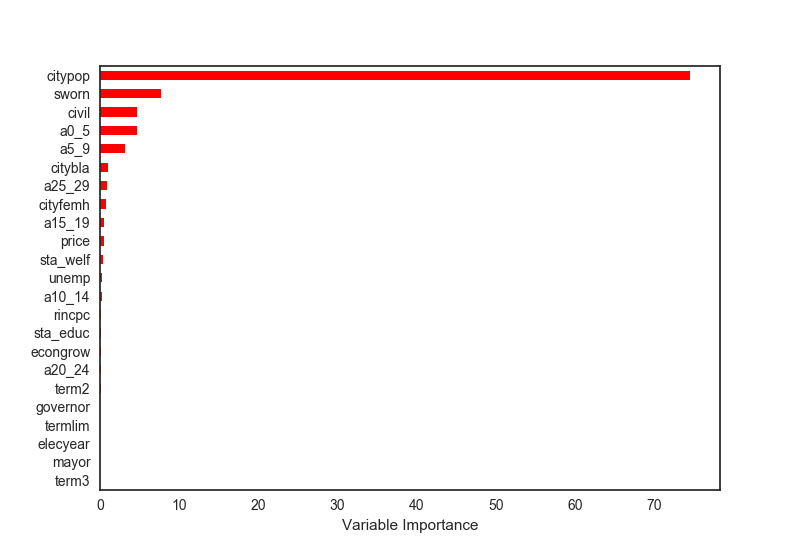
\includegraphics[width=.8\linewidth,height=4cm]{crime_randtu}
  \captionof{figure}{Importance\\ from random forest}
  \label{fig:test2}
\end{minipage}
\end{figure}


\subsection{Boosting and Random Forest}
To optimize the results from the regression tree, we tried random forest and gradient boosting methods. We found that gradient boosting gives a testing error of 0.04 and random forest using all features further reduces the results to 0.02. To compare the reason we plot the variable importance which indicates the reduction in Gini index if we eliminate this variable, and as shown random forest gives a good indication that \textit{citypop} is the dominating feature. So in such kind of data where only one feature dominates, we can see that the Random Forest performs better.

\subsection{Remarks}
Despite tree-based methods generally perform better in the crime dataset, we can not yet conclude that tree-based methods would always perform better, since crime data is low dimension with only very few important features and they have different importance, and tree-based methods can intuitively perform well in such cases. It remains to see the results in the in-Kaggle competition, whose data has some different features.


\section{The Combinatorial Drug 20 Efficacy Data}
\label{combodrug}
\subsection{Data Description}

The dataset contains 120 sample cell lines with 21 attributes in total and 20 instances are hidden for testing purpose. D1, D2, ..., D20 are 20 discrete features indicating random 4-level combinations of 20 types of drugs. The only real-valued attribute is the viability difference \footnote{Viability difference = normal cell - cancer cell, also known as therapeutic window.}, which is the response variable in this study.  Higher viability value implicates better efficacy of the drug combo.

\subsection{Tree-based Model Analysis}
\subsubsection{Regression Tree}
We performed regression tree analysis on the whole training dataset first and obtained a complicated regression tree with depth equal to 9.
However, after we utilized 5-fold cross validation to simplify the tree and minimize the deviance related, we obtained a pruned tree with one split only.
From the figure shown below, D3 is the variable with highest importance and thus the dataset actually has two main clusters separated by D3. However, despite from the intepretability, the cross-validation mean squared error of simple regression tree is indeed not satisfactory. After tree pruning, the overfitting problem was alleviated but the simple pattern of the pruned tree indicated that significant information loss exists in this model. 



\begin{figure}[h]
  \centering
  \fbox{
  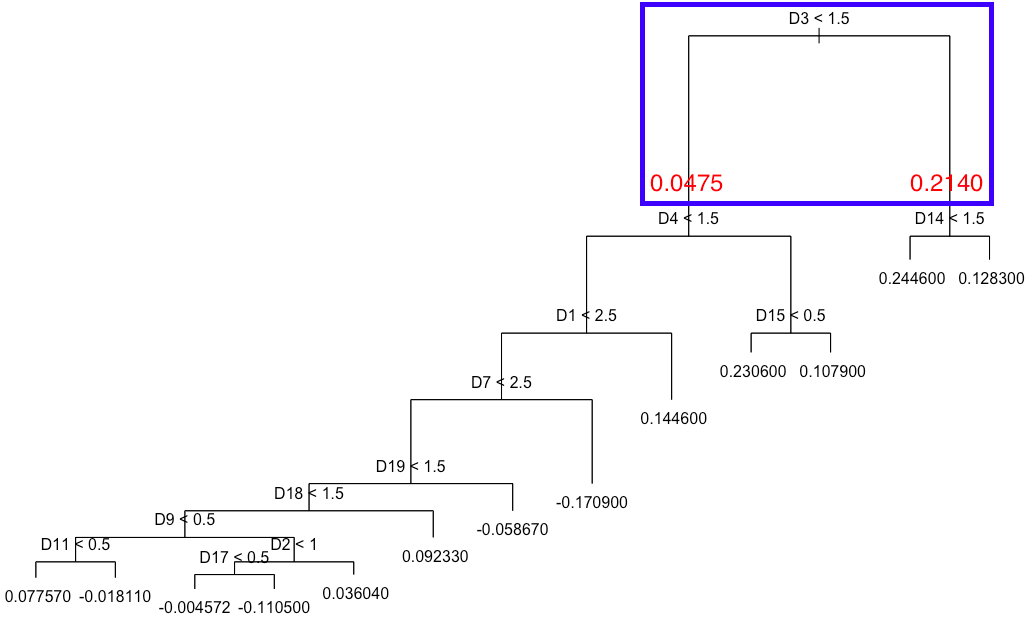
\includegraphics[height = 8cm]{combo_tree1}
  }
  \caption{Full regression tree v.s. the pruned tree (within blue rectangle).}
\end{figure}

\subsubsection{Bagging and Random Forest}
Due to the high intepretability of tree-based method but low prediction power, in this part we aim to check whether Bagging and Random Forest can be used to mitigate this problem and enhance the prediction power.
Regression tree methods suffer a lot from high variance. Bootstrap aggregation for training datasets is one crucial technique for variance reduction. In this dataset, the number of instances = 100, which is moderately larger than the number of attributes = 20, so we expect that the variance reduction through random forest an bagging can be effective.
In theory, random forest is expected to perform better than bagging because of decorrelation between random trees.
Random forest achieves better variance reduction by reducing the predictor subset size. Three classical choice of the number of predictors are: $p, p/3, \sqrt{p}$. Therefore, we implement the random forest function three times with $mtry = 20, 7, 4$ respectively. Variable importance measure plots also show that D3 dominates other variables.

\subsubsection{Boosting}
Boosting to regression trees is another approach to improve the prediction accuracy. A large number of trees are built sequentially based on previous trees in order to fit the residuals iteratively. For this dataset, we set the shrinkage parameter $\lambda = 0.001$ small enough and the number of trees = 5000 to ensure the generalized boosted model is well learned. Aftering implementing the boosted model with $interaction\_depth = 1$ and the one with $interaction\_depth = 4$, the results are within our expectation. Both training error and CV error do not differ much after making the trees more complicated, which coincides with the one-split pruned tree previously mentioned.

\subsubsection{Comparison with Linear Model}
In order to compare tree-based models with linear models, we implemented Ridge and Lasso regression. Optimal shrinkage parameters are selected to minimize the 5-fold cross validation mean squared error. For Ridge, $\lambda_{Ridge}^{\star} = 0.02702$ and $MSE_{Ridge} = 0.01345$; For Lasso, $\lambda_{Lasso}^{\star} = 0.00864$ and $MSE_{Lasso} = 0.01352$.

\subsection{Results and Discussion}
This combinatorial drug 20 efficacy data is a typical dataset example with real-valued output and discrete inputs. According to the trade-off between interpretability and prediction accuracy,  linear models are usually expected to have better performance than simple regression tree. More advanced tree-based methodologies may improve the accuracy significantly.\\

The original regression tree, which has tree depth equal to 9, suffers from overfitting problem with poor cross validation MSE. Although the pruned tree only involves D3, it outperforms the full regression tree anyway. The Kaggle testing MSE for pruned tree can reach 0.01655.\\

Bagging, as well as Random Forests, achieves excellent performance with respect to data training as shown in the result table. In terms of Kaggle testing, bagging and random forest (number of variables considered when splitting = 7) achieve a MSE = 0.01066 and a MSE = 0.01079 respectively. However, the percentage of variances explained by both approaches only range around $20\%$. Better techniques are needed to explain more of this dataset. From the perspective of decorrelation between individual trees, one may expect that Random Forests should display dominant patterns over Bagging according to the theory. A possible explanation would be 

\begin{figure}[h]
  \centering
  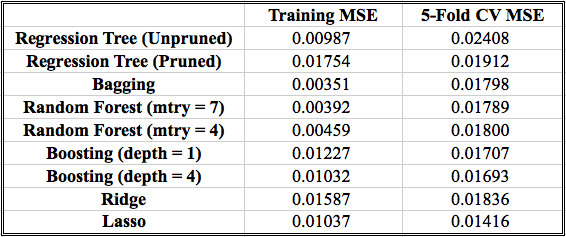
\includegraphics[height = 4cm]{combo_result}
  \caption{Comparison between selected models.}
\end{figure}


\newpage
\section{Results of Binary OneDrug}
\label{drug2}
In Section \ref{combodrug}, we have seen that, tree-based models have relatively satisfactory performance for discrete-valued input and real-valued output data. To further evaluate their robustness for similar dataset, we applied these tree-based models on the in-class Kaggle Competition: Binary DrugSensitivity2 to "compete" with other students' regression models.\\

In this section, we will first present results of Bagging, Random Forest and Boosting models on validation set. Then we will see how they perform on test set, i.e. in-class competition with ground truth. Since Section \ref{combodrug} has discussed a lot on the theory of tree-based models with similar dataset, we will not focus on the theoretical part but try to give straight results on these models. 
 
\subsection{Data Description}
The OneDrug dataset contains 642 cancer cell line samples, with 60 binary features as gene mutation status and 1 real-valued response, logarithmic IC50, to measure drug sensitivity. The basic problem is to predict the responses of these test samples based on their binary predictors/features.

We are interested in the following 4 tree-based models:
\begin{itemize}
	\item Bagging
	\item Random Forest with $mtr = \sqrt{p}$ 
	\item Random Forest with a fixed-value $mtr$
	\item Boosting with $depth = 1$
\end{itemize}

\subsection{Results on Validation Set}
\begin{figure}[h]
	\centering
	\fbox{
		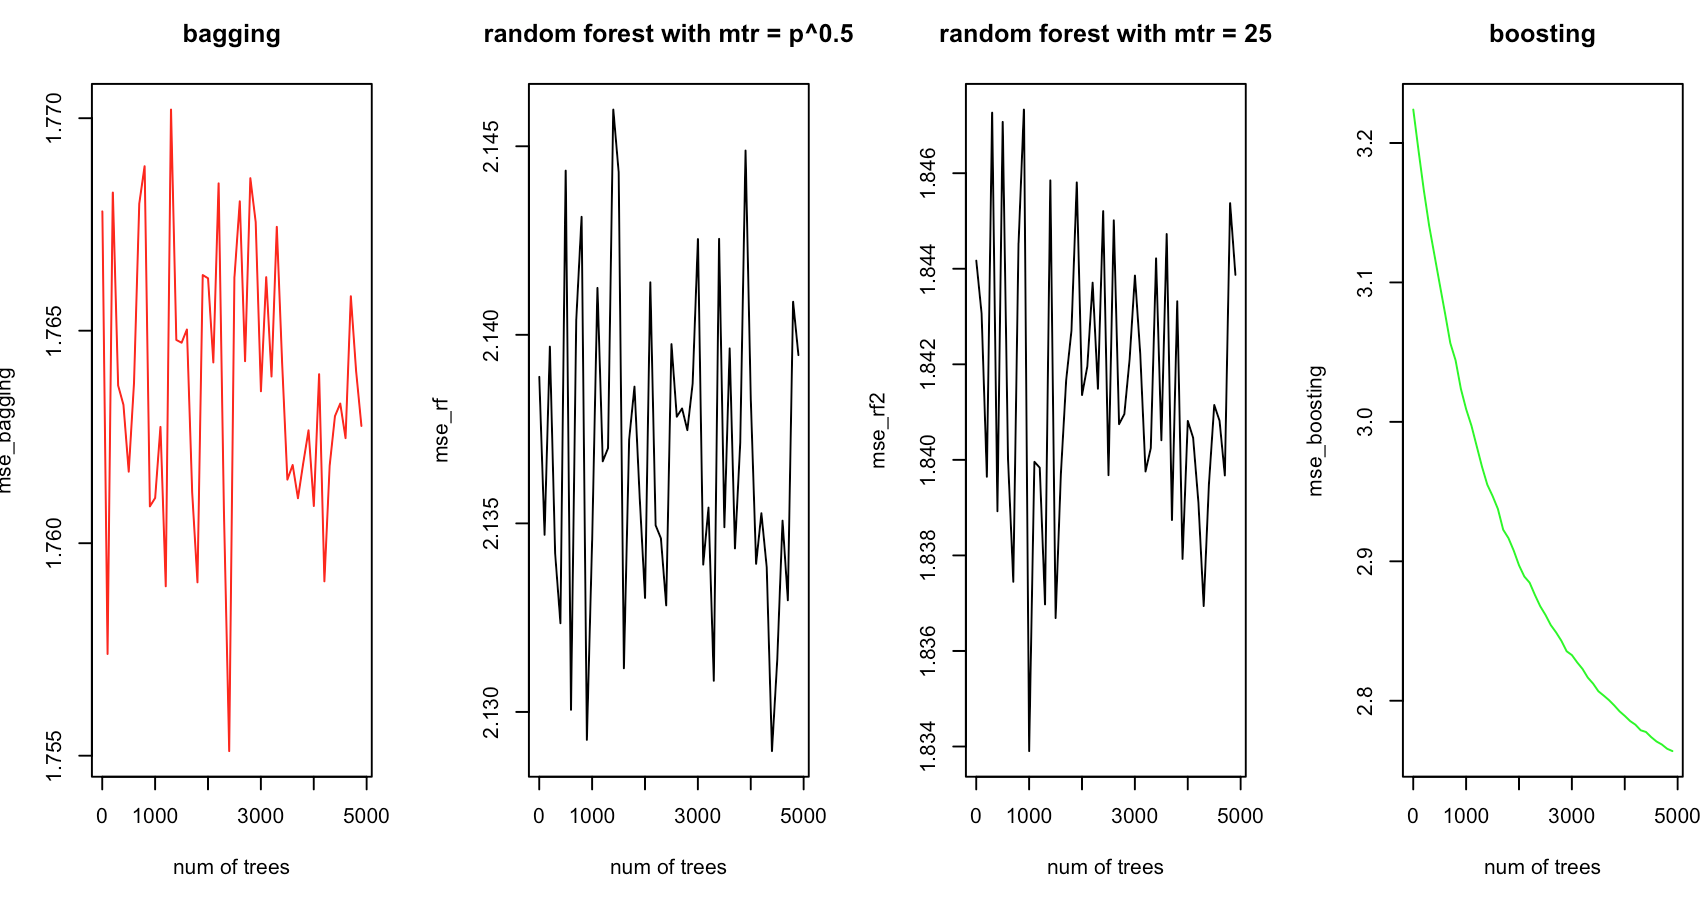
\includegraphics[height = 8cm]{drug_validation}
	}
	\caption{Mean Squared Error (MSE) v.s. Number of Trees}
\end{figure}

For this OneDrug dataset, except for the boosting model, it might be hard to observe the relationship between $MSE$ and \textit{Number of Trees}, but we are still able to see that, for this dataset, bagging performs better in the validation step. But what about in the test (Kaggle ground truth) set?

\clearpage
\subsection{Results on Test Set: Kaggle Competition}
\begin{table}[h!]
	\centering
	\caption{Kaggle $MSE$ \& Ranking}
	\label{my-label}
	\begin{tabular}{|l|l|l|}
		\hline
		Model                                                & Kaggle MSE & Ranking (until 9 April, 2017) \\ \hline
		Bagging, 5000 trees                                  & 3.13505    & 7th                           \\ \hline
		Random Forest with $\sqrt{p}$, 5000 trees & 3.15232    & 8th                           \\ \hline
		Random Forest with a fixed $mtr$, 5000 trees           & 3.09702    & 3th                           \\ \hline
		Boosting, 5000 trees                                 & 3.23300    &                               \\ \hline
	\end{tabular}
\end{table}

\section{Conclusion}
\label{con}
In this second mini-project, we apply several tree-based models 

\subsubsection*{Acknowledgments}
\section*{References}
\small
[1] Alexander, J.A.\ \& Mozer, M.C.\ (1995) Template-based algorithms
for connectionist rule extraction. In G.\ Tesauro, D.S.\ Touretzky and
T.K.\ Leen (eds.), {\it Advances in Neural Information Processing
  Systems 7}, pp.\ 609--616. Cambridge, MA: MIT Press.
\end{document}
